\section{Ejercicio 3: El retorno del jedi}

    % Describir detalladamente el problema a resolver dando ejemplos del mismo y sus soluciones.
    \subsection{Descripción del problema}

    \begin{figure}[ht]
        \begin{center}
            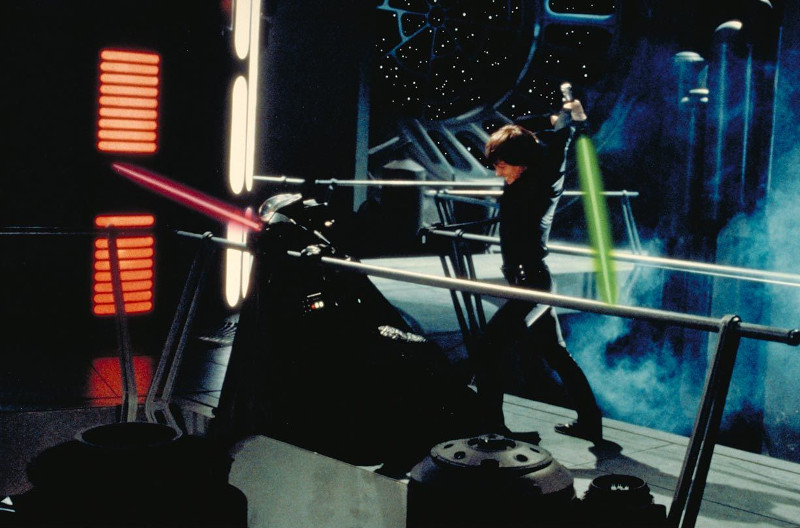
\includegraphics[width=10cm]{imagenes/el_retorno_del_jedi.jpg}
			\caption*{``Muchos son los caminos que conllevan al lado oscuro, el
			odio lleva a la ira, la ira lleva a la venganza''.}
        \end{center}
    \end{figure}

	Luke debe enfrentar a su padre. Para ello debe moverse por una grilla,
	arrancando en la esquina superior izquierda para terminar en la opuesta,
	donde aguarda Darth Vader. Cada casilla de la grilla tiene una altura
	asociada, donde dependiendo de la diferencia en altura entre el casillero
	actual de Luke y su destino le costará más o menos energía moverse. Además
	se tiene la condición de que Luke únicamente puede avanzar hacia abajo o
	hacia la derecha, dado que considera un acto de cobardía retroceder sobre
	sus pasos. El objetivo es encontrar y devolver el camino donde Luke gasta la
	menor cantidad de energía en alcanzar su destino.

	Formalizando el problema, se tiene una grilla $G$ rectangular de dimensiones $N \times
	M$ donde Luke comienza en la posición $(1, 1)$ y desea llegar a $(N, M)$.
	Sea $G_{ij}$ con $1 \leq i \leq N$ y $1 \leq j \leq M$ la altura de cada
	casillero, $H$ el nivel de entrenamiento de Luke y $\Delta$ la
	diferencia de altura entre el casillero actual y el próximo, el costo de
	energía para cada movimiento se calcula de la siguiente manera: nulo si $|\Delta|
	\leq H$, $|\Delta| - H$ en caso contrario. La condición de que Luke no pueda
	retroceder es equivalente a decir que únicamente puede moverse de forma
	creciente en $i$ o $j$.

	El formato de entrada para el problema es el siguiente, donde la primer
	línea posee las dimensiones de la grilla y el nivel de entrenamiento de
	Luke, y las siguientes $N$ entradas contienen $M$ elementos donde cada uno
	representa la altura del casillero correspondiente.

	~
	\begin{center}
		\begin{tabular}{cccc}
			$N$ & $M$ & $H$ & \\
			$G_{11}$ & $G_{12}$ & $\dots$ & $G_{1M}$ \\
			$G_{21}$ & $G_{22}$ & $\dots$ & $G_{2M}$ \\
			$\vdots$ & & & \\
			$G_{N1}$ & $G_{N2}$ & $\dots$ & $G_{NM}$ \\
		\end{tabular}
	\end{center}

	~

	La salida está compuesta por una primer línea con el costo del camino
	seleccionado y $N + M - 2$ líneas con la dirección ($X$ o $Y$) a tomar en cada paso para
	realizar el mismo. Cabe aclarar que $X$ implica avanzar una filas e $Y$
	una columna.

	A continuación se presenta un ejemplo de entrada con su salida
	correspondiente:

	~

	\begin{figure}[H]
		\centering
		\begin{minipage}[t]{0.25\textwidth}
			\begin{tabular}[t]{ccc}
				\multicolumn{3}{l}{\textbf{Entrada}} \\
				\texttt{3} & \texttt{3} & \texttt{1} \\
				\texttt{4} & \texttt{-2} & \texttt{-1} \\
				\texttt{6} & \texttt{7} & \texttt{-5} \\
				\texttt{0} & \texttt{3} & \texttt{4} \\
			\end{tabular}
		\end{minipage}
		\begin{minipage}[t]{0.10\textwidth}
			\begin{tabular}[t]{l}
				\textbf{Salida} \\
				\texttt{4} \\
				\texttt{X} \\
				\texttt{Y} \\
				\texttt{X} \\
				\texttt{Y} \\
			\end{tabular}
		\end{minipage}
	\end{figure}

	\begin{figure}[H]
		\centering
		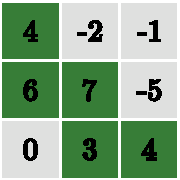
\includegraphics{imagenes/ej3_grilla_1.pdf}
		\caption{Camino de menor costo.}
	\end{figure}

    % Explicar de forma clara, sencilla, estructurada y concisa, las ideas desarrolladas para la resolución del problema. Utilizar pseudocódigo y lenguaje coloquial (no código fuente). Justificar por qué el procedimiento resuelve efectivamente el problema.
    \subsection{Solución propuesta}

	Para la resolución de este ejercicio se utilizó programación dinámica dado
	que el mismo presenta solapamiento de subproblemas y es posible definir una
	formulación recursiva que lo resuelva haciendo uso del principio de
	optimalidad.

	Dada una entrada con entrenamiento $H$, la siguiente función modela la solución al
	problema:

	\begin{equation*}
		f(N, M) = \text{Costo mínimo de $(1, 1)$ a $(N, M)$ para Luke con entrenamiento $H$}
	\end{equation*}

	Luego se plantea la recurrencia donde es posible visualizar qué valores
	podrían guardarse para no tener que recalcularlos (solapamiento).
	Antes por comodidad se define la siguiente función $g$ para calcular el costo de cada salto:

	\begin{equation*}
		g(i, j, i', j') =
		\begin{cases}
			|G_{ij} - G_{i'j'}| - H & \text{si } |G_{ij} - G_{i'j'}| > H \\
			0 & \text{caso contrario}
		\end{cases}
	\end{equation*}

	Ahora sí se define la versión recursiva del ejercicio de la siguiente manera:

	\begin{align*}
		f(1, 1) &= 0 \\
		f(1, j) &= g(1, j, 1, j - 1) + f(1, j - 1) \\
		f(i, 1) &= g(i, 1, i - 1, 1) + f(i - 1, 1) \\
		f(i, j) &= \text{mín}\left \{ f(i - 1, j) + g(i, j, i - 1, j), f(i, j - 1) + g(i, j, i, j - 1) \right \} \\
	\end{align*}

	Esta recurrencia es una solución al problema únicamente si se cumple el principio
	de optimalidad. Si el mismo se cumple, entonces las subsoluciones al problema son
	óptimas, pudiendo así operar y reutilizar valores que se tiene la certeza
	que son el mejor camino a tomar. Los subproblemas para este ejercicio están
	representados por el costo mínimo hasta cualquier $(i, j)$ dado por $f(i,
	j)$. Por lo tanto a continuación se procederá a demostrar que vale tal
	propiedad.

	\subsubsection*{Optimalidad de subproblemas}

	La idea detrás de la recurrencia es que la solución de encontrar el camino
	de menor costo hasta $(N, M)$ se puede pensar como la decisión entre tomar
	el mejor camino a $(N - 1, M)$ o $(N, M - 1)$ más el salto final. Para poder
	usar esto es necesario entonces demostrar que el camino seleccionado hasta
	$(N - 1, M)$ o $(N, M - 1)$ sea óptimo.

	Este es el concepto de subproblemas, el hecho de considerar todo camino a
	$(i, j)$ como una subsolución al problema principal. Para probar que con la
	función recursiva se obtienen estas subsoluciones óptimas se realiza
	inducción sobre $N$ y $M$.

	~

	\textbf{Caso base: } $N = M = 1$

	Por definición de la recurrencia, $f(1, 1) = 0$ lo cual es válido ya que si
	Luke no tiene que moverse en ninguna dirección, no necesita realizar ningún
	salto manteniendo intacto su nivel de energía. Queda así demostrada la
	validez del caso base.

	~

	\textbf{Paso inductivo}

	Para el paso inductivo es necesario contemplar por separado los casos
	bordes, con lo cual se analizarán tres situaciones posibles.

	\begin{enumerate}
		\item{
			\textbf{Columna lateral izquierda: } $f(i, 1)$ con $1 < i < N$

			Como hipótesis inductiva, se asume $f(i - 1, 1)$ óptimo.

			Luke únicamente puede avanzar en orden creciente tanto en $i$
			o en $j$, la única forma de acceder a los casilleros de la primer
			columna es avanzando sólo en $i$, ya que en con moverse
			una posición en $j$ ya le resulta imposible retroceder y llegar a
			estos.

			Estos caminos están definidos por $f(i, 1) = g(i, 1, i - 1, 1) + f(i
			- 1, 1)$ donde se toma el costo del camino hasta una posición atrás
			en $i$ y se le suma el valor del salto. Como sólo es posible llegar
			a través del casillero anterior ($i - 1$, 1), y por hipótesis inductiva
			dijimos que $f(i - 1, 1)$ era óptimo, al sumarle el valor del salto
			se obtiene la subsolución $f(i, 1)$.
		}
		\item{
			\textbf{Fila superior: } $f(1, j)$ con $1 < j < M$

			Como hipótesis inductiva, se asume $f(1, j - 1)$ óptimo.

			Similar al punto anterior, por la restricción que tiene Luke para
			desplazarse, estas posiciones sólo pueden accederse avanzando sólo
			en $j$ desde el casillero inicial.

			Los costos están definidos por $f(1, j) = g(1, j, 1, j - 1) + f(1, j
			- 1)$, que toma el costo del camino hasta una posición atrás en $j$
			y le suma el valor del salto. Dado que sólo es posible llegar desde
			$(1, j - 1)$ y por hipótesis inductiva $f(1, j - 1)$ es óptimo, al
			sumarle el salto se obtiene la subsolución $f(1, j)$.
		}
		\item{
			\textbf{Elementos restantes: } $f(i, j)$ con $1 < i \leq N$ y $1 < j \leq M$

			Como hipótesis inductiva, se asumen $f(i - 1, j)$ y $f(i, j - 1)$
			óptimos.

			Habiendo considerado ya los casos bordes, ahora es posible para el
			resto de casilleros $(i, j)$ dar su camino de menor costo, ya que
			para llegar a uno de ellos hay sólo dos opciones: se salta de $(i -
			1, j)$ o de $(i, j - 1)$. Luke no puede moverse en diagonal ni
			retroceder en $i$ o en $j$ con lo cual lo que resta es ver cuál de
			estos caminos le conviene más.

			Por hipótesis inductiva se tenía que $f(i - 1, j)$ y $f(i, j - 1)$
			eran costos óptimos, con lo cual tomando la definición de la
			recursión para estos casos:

			$f(i, j) = \text{mín}\left \{ f(i - 1, j) + g(i, j, i - 1, j), f(i, j - 1) + g(i, j, i, j - 1) \right \}$

			Podemos observar que se busca entre estos dos caminos el que al
			sumarle el costo del salto sea mínimo. Entonces podemos afirmar que
			la elección que toma para $(i, j)$ es la mejor, ya que la
			alternativa resulta en un camino que es igual o peor. Por lo tanto
			demostramos así que vale la optimalidad de la subsolución $f(i, j)$.

		}
	\end{enumerate}

	Se concluye por inducción sobre $N$ y $M$ que para todo $(i, j)$ con $1 \leq
	i \leq N$ y $1 \leq j \leq M$, $f(i, j)$ es una subsolución óptima. En
	particular, tomando $f(N, M)$ se obtiene el costo mínimo del problema
	planteado.

	Es así como se demuestra que vale el principio de optimalidad para el
	ejercicio dado con la formulación recursiva planteada, probando entonces que
	nos presenta una solución válida al mismo.

	\subsubsection{Implementación}

	Para la implementación de esta formulación recursiva había dos caminos
	posibles. Una era implementar la recursión tal cual como está definida,
	también denominada como una implementación \emph{top-down}, donde al llamar a $f(N,
	M)$ se abre el árbol de recursiones para $f(N - 1, M)$ y $f(N, M - 1)$
	respectivamente, yendo de los problemas más grandes a los más pequeños. Por
	otro lado estaba \emph{bottom-up}, que a diferencia del primero, comienza
	calculando los subproblemas más pequeños para luego ir construyendo los más
	grandes.

	La implementación \emph{top-down} hubiera resultado, donde para aprovechar
	el solapamiento de subproblemas se podrían haber almacenado los valores de
	las llamadas recursivas que se iban calculando. Sin embargo, los algoritmos
	recursivos presentan un \emph{overhead} a la hora de ejecutarse y corren
	riesgo de quedarse sin lugar en la pila.

	Con \emph{bottom-up}, también se resuelve el solapamiento de subproblemas
	guardando los valores de los mismos, con la diferencia de que se los calcula
	explícitamente. Esto significa que a diferencia de la versión recursiva
	donde los mismos se almacenan luego de haber resuelto la llamada recursiva,
	aquí se calculan y guardan de forma iterativa. Para esto, el mismo debe
	contar con que se cumplan las dependencias de cada subproblema que resuelve.

	Se optó por realizar una implementación \emph{bottom-up} dado que la
	complejidad asintótica resulta la misma que con \emph{top-down} sólo que sin el peligro
	de quedarse sin espacio en la pila.

	Con respecto a la resolución de dependencias, el secreto está en el orden en
	el cual se van resolviendo los subproblemas. Para este ejercicio, cada
	subproblema $(i, j)$ requiere ya tener calculados $(i - 1, j)$ y $(i, j -
	1)$. Existen varias formas de ir calculando los valores y que se cumpla esta
	dependencia, para la implementación desarrollada en este trabajo se decidió
	tomar la de calcular la primer fila de izquierda a derecha, la primer
	columna de arriba a abajo y luego el resto de las filas de izquierda a
	derecha.

	En el gráfico a continuación se puede observar el comportamiento descrito,
	donde los casilleros oscuros son el camino a calcular y los que poseen
	asteriscos sus dependencias.

	\begin{figure}[H]
		\centering
		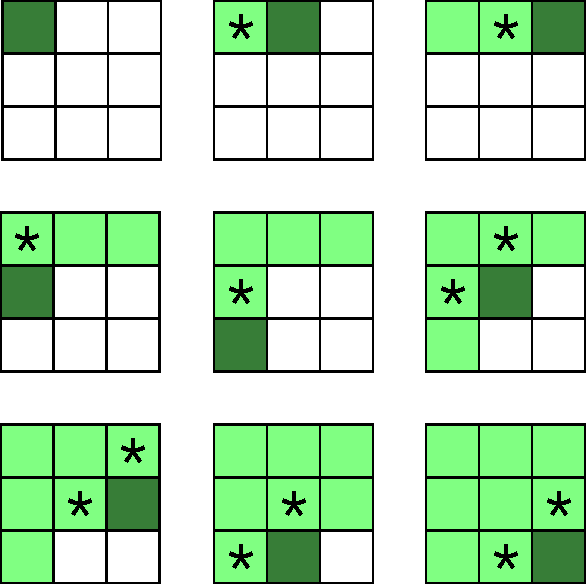
\includegraphics{imagenes/ej3_grilla_2.pdf}
		\caption{Visualización del cálculo de subsoluciones.}
	\end{figure}

	Por último, una vez que se tienen los valores finales de todos los
	casilleros calculados, se desea generar el camino buscado.

	Primero es necesario destacar que para cada posición de la
	grilla (además del costo) se guarda la dirección: \texttt{Y} corresponde a
	un salto horizontal, \texttt{X} vertical. De esta forma, al momento de
	construir el recorrido final, lo que se busca es tomar la dirección en la
	posición $(N, M)$ y dependiendo de la misma continuar el proceso
	en el casillero correspondiente ($(N, M - 1)$ si fuera \texttt{Y}, $(N - 1,
	M)$ caso contrario) guardando en cada paso la dirección tomada.

	Al finalizar se obtiene una secuencia con la dirección a tomar
	en cada paso para obtener el recorrido de costo óptimo.

	Todos los pasos descritos anteriormente se llevan a cabo mediante el siguiente algoritmo:

	\begin{algorithm}[H]
		\caption{Solución \emph{bottom-up} al problema}
		\Input{Una grilla $G$ de dimensiones $N \times M$ con la altura de cada
		casillero y un nivel de entrenamiento $H$.}
		\Output{Un par con el costo del camino óptimo de $(1, 1)$ a
		$(N, M)$ y su recorrido.}
		$DP$ $\gets$ grilla de dimensiones $N \times M$ donde cada elemento es
		un par del tipo entero y caracter \;
		$DP_{1,1}$ $\gets$ (0, 'I') \;
		\ForEach{$i$ entre $2$ y $N$}{
			$DP_{i,1}$ $\gets$ ($DP_{i-1,1} + $ costo del salto vertical, 'X') \;
		}
		\ForEach{$j$ entre $2$ y $M$}{
			$DP_{1,j}$ $\gets$ ($DP_{1,j-1} + $ costo del salto horizontal, 'Y') \;
		}
		\ForEach{$i$ entre $2$ y $N$ y $j$ entre $2$ y $M$}{
			$costoSaltoVertical$ $\gets$ $DP_{i-1,j} + $ costo del salto vertical \;
			$costoSaltoHorizontal$ $\gets$ $DP_{i,j-1} + $ costo del salto horizontal\;
			\eIf{$costoSaltoVertical < costoSaltoHorizontal$}{
				$DP_{i,j}$ $\gets$ ($costoSaltoVertical$, 'X') \;
			}
			{
				$DP_{i,j}$ $\gets$ ($costoSaltoHorizontal$, 'Y') \;
			}
		}
		$i$ $\gets$ $N$ \;
		$j$ $\gets$ $M$ \;
		$k$ $\gets$ $N + M - 2$ \;
		\While{$k > 0$}{
			$camino_k$ $\gets$ $DP_{i,j}$.segundo() \;
			\eIf{$DP_{i,j}$.segundo() es igual a 'Y'}{
				$j$ $\gets$ $j - 1$ \;
			}
			{
				$i$ $\gets$ $i - 1$ \;
			}
			$k$ $\gets$ $k - 1$ \;
		}
		\Return{($DP_{N,M}$, $camino$)}
	\end{algorithm}

    % Deducir una cota de complejidad temporal del algoritmo propuesto (en función de los parámetros que se consideren correctos) y justificar por qué el algoritmo la cumple. Utilizar el modelo uniforme.
    \subsection{Complejidad teórica}
	Inicializar la matriz de subsoluciones $DP$ de $N$ filas y $M$ columnas
	tiene un costo de $\ord(N \times M)$.

	Calcular el salto vertical u horizontal tiene un costo de $\ord(1)$.
	Calcular la primera fila tiene costo $\ord(M)$, ya que crece únicamente en
	función del tamaño de la fila la cantidad de operaciones constantes
	necesarias para calcular y almacenar en la matriz de subsoluciones ($DP$).
	Calcular la primera columna cuesta $\ord(N)$, ya que crece únicamente en
	función del tamaño de la columna el número de operaciones constantes
	necesarias.

    Para llenar el resto de la grilla $DP$, se la debe recorrer en orden creciente por columnas, a partir de la segunda fila y desde la segunda columna. En cada iteración se toma el mínimo entre dos valores: el costo del salto vertical más la subsolución correspondiente a la posición de arriba en la grilla, y el costo del salto horizontal más la subsolución correspondiente a la posición de la izquierda. Todas estas operaciones tienen un costo de $\ord(1)$, dando una complejidad total para terminar de llenar la grilla $DP$ de $\ord(N \times M)$.

    Para armar el camino, se va recorriendo la matriz desde la posición final, (fila $N - 1$ , columna $M - 1$) hasta la inicial (fila $0$ , columna $0$); en cada paso se consulta en la matriz $DP$ la dirección del movimiento correspondiente, se lo almacena, y se mueve a la siguiente posición (operaciones $\ord(1)$). Esto se repite un total de $N + M - 2$ iteraciones, ya que en cada paso corresponde a un movimiento a la izquierda o hacia arriba. Entonces, armar el camino cuesta $\ord(N + M - 2)$

    Por lo tanto, el costo total es $\ord( M + N + M \times N + (N + M - 2) ) = \ord(N \times M)$

    \subsection{Experimentación}
    El objetivo de la experimentación fue ver que la solución depende linealmente con respecto a $N$ y a $M$ y no depende de $H$.

    Para esto se realizaron cuatro experimentos:
    \begin{itemize}
        \item Variar $N$: Se varía entre 1 y 50000, con saltos de a 200 ($T_N$).
        \item Variar $M$: Se varía entre 1 y 50000, con saltos de a 200 ($T_M$).
        \item Variar $N$ y $M$: Se varía entre 1 y 1000, con saltos de a 10 ($T_{M \times N}$), $N$ y $M$ toman el mismo valor.
        \item Variar $H$: Se varía entre 1 y 50000, con saltos de a 200 ($T_H$), fijando el $M$ y el $N$ en $50000$.
    \end{itemize}
    En todos estos experimentos, el contenido de cada casilla de la matriz
    fue elegido aleatoriamente.

    \subsubsection{Resultados}

    \begin{figure}[H]
        \centering
        \begin{tikzpicture}
            \begin{axis}[
                    title={},
                    xlabel={Cantidad de filas ($N$) o de columnas ($M$)},
                    ylabel={Tiempo de ejecución (nanosegundos)},
                    scaled x ticks=false,
                    scaled y ticks=false,
                    enlargelimits=0.05,
                    width=0.5\textwidth,
                    height=0.5\textwidth,
                    legend pos=north west,
                    legend cell align=left,
                    xmin=100
                ]
                \addplot[color=green] table[x index=0,y index=1]{../exp/elRetornoDelJediFilas};
                \addplot[color=blue] table[x index=0,y index=1]{../exp/elRetornoDelJediColumnas};
                \addplot[color=red] table[x index=0, y expr={x*70}]{../exp/elRetornoDelJediFilas};
                \addplot[color=violet] table[x index=0, y expr={x*10}]{../exp/elRetornoDelJediColumnas};
                \legend{$T_N$,$T_M$, $c_1 \times N$, $c_2 \times M$}
            \end{axis}
        \end{tikzpicture}
        \caption{Tiempos de ejecución observados al variar los valores de $M$
        ($T_M$) y de $N$ ($T_N$). Se considera $c_1 = 70$ y $c_2 = 10$.}
        \label{fig:exp3:var-nym-base}
    \end{figure}

	En el gráfico de la Figura \ref{fig:exp3:var-nym-base} se puede ver que al 
	variar el valor de $N$, $T_N$  es acotable por por una recta con constante 
	$c_1$ y al variar $M$, $T_M$ es acotable por una recta con constante $c_2$, lo 
	cual prueba empíricamente la hipótesis de que la complejidad del algoritmo 
	tiene una relación lineal con los valores tanto de $M$ como de $N$. 
	Las rectas $T_N$ y $T_M$ difieren en la constante; esto se
	debe a las estructuras de datos utilizadas durante la resolución, ya que al
	aumentar el valor de $M$ se utiliza siempre un único vector grande, mientras
	que, al aumentar el $N$ se tienen $N$ vectores con un único elemento, lo
	cual hace que acceder al $i$-ésimo vector pueda volverse un poco más
	costoso, por ejemplo, porque los vectores podrían estar almacenados en
	lugares no contiguos de memoria.

    \begin{figure}[H]
        \centering
        \begin{tikzpicture}
            \begin{axis}[
                    title={},
                    xlabel={Cantidad de filas ($N$) o de columnas ($M$), para $c = 70$},
                    ylabel={Tiempo de ejecución (nanosegundos)},
                    scaled x ticks=false,
                    scaled y ticks=false,
                    enlargelimits=0.05,
                    width=0.5\textwidth,
                    height=0.5\textwidth,
                    legend pos=north west,
                    legend cell align=left,
                    restrict x to domain=2000:50000,
                    ymax=100,
                    xmin=1
                ]
                \addplot[color=green] table[x index=0,y expr={\thisrowno{1}/x}]{../exp/elRetornoDelJediFilas};
                \addplot[color=blue] table[x index=0,y expr={\thisrowno{1}/x}]{../exp/elRetornoDelJediColumnas};
                \addplot[color=red] table[x index=0, y expr={70}]{../exp/elRetornoDelJediFilas};
                \addplot[color=violet] table[x index=0, y expr={10}]{../exp/elRetornoDelJediFilas};
                \legend{$T_N/N$,$T_M/M$,$c_1$,$c_2$}
            \end{axis}
        \end{tikzpicture}
        \caption{Cociente entre los tiempos de ejecución observados, $T_M$ y
        $T_N$ y los valores correspondientes de $M$ y de $N$, respectivamente.
        Se considera $c_1 = 70$ y $c_2 = 10$.}
        \label{fig:exp3:var-nym-divconst}
    \end{figure}


	En el gráfico de la Figura \ref{fig:exp3:var-nym-divconst}, se puede ver que
	si se lo divide por $N$ o $M$, el tiempo de ejecución de $T_N$ queda acotable 
	por $c_1$ y $T_M$ por $c_2$ , lo cual confirma sus linealidades  .
	\begin{figure}[H]
        \centering
        \caption{}
        \label{fig:exp3:var-nxn-base}
        \begin{tikzpicture}
            \begin{axis}[
                    title={},
                    xlabel={Tamaño de entrada ($N = M$)},
                    ylabel={Tiempo de ejecución (nanosegundos)},
                    scaled x ticks=false,
                    scaled y ticks=false,
                    enlargelimits=0.05,
                    width=0.5\textwidth,
                    height=0.5\textwidth,
                    legend pos=north west,
                    legend cell align=left,
                    xmin=1
                ]
                \addplot[color=black] table[x index=0,y index=1]{../exp/elRetornoDelJediFilasYColumnas};
                \addplot[color=red] table[x index=0, y expr={x*x*20}]{../exp/elRetornoDelJediFilasYColumnas};
                \legend{$T_{M \times N}$, $cN^{2}$}
            \end{axis}
        \end{tikzpicture}
        \caption{Tiempos de ejecución observados al variar los valores de $N$
        ($T_{M \times N}$) . Se considera $c = 20$ .}
    \end{figure}

	En la Figura \ref{fig:exp3:var-nxn-base} se puede ver que al variar el $N$
	(y simultáneamente el $M$, ya que se considera $M = N$), $T_{M \times N}$ se
	puede acotar por una función cuadrática con constante $c$.  

	Dadas las irregularidades en $T_{M \times N}$, se corrió el mismo escenario 
	varias veces para analizar dichos picos.

	\begin{figure}[H]
        \centering
        \caption{}
        \label{fig:exp3:var-nxn-divconst}
        \begin{tikzpicture}
            \begin{axis}[
                    title={},
                    xlabel={Tamaño de entrada ($N$)},
                    ylabel={Tiempo de ejecución (nanosegundos)},
                    scaled x ticks=false,
                    scaled y ticks=false,
                    enlargelimits=0.05,
                    width=0.5\textwidth,
                    height=0.5\textwidth,
                    legend pos=north west,
                    legend cell align=left,
                    restrict x to domain=5:1000,
                    xmin=100
                ]
                \addplot[color=black,only marks] table[x index=0,y index=1]{../exp/elRetornoDelJediFilasYColumnas1};
                \addplot[color=red,only marks] table[x index=0,y index=1]{../exp/elRetornoDelJediFilasYColumnas2};
                \addplot[color=blue,only marks] table[x index=0,y index=1]{../exp/elRetornoDelJediFilasYColumnas3};
                \addplot[color=violet,only marks] table[x index=0,y index=1]{../exp/elRetornoDelJediFilasYColumnas4};
                \addplot[color=green,only marks] table[x index=0,y index=1]{../exp/elRetornoDelJediFilasYColumnas5};
               \legend{$T_{M \times N}_1$, $T_{M \times N}_2$,$T_{M \times N}_3$,$T_{M \times N}_4$,$T_{M \times N}_5$}
            \end{axis}
        \end{tikzpicture}
        \caption{Tiempos de ejecución observados al variar los valores de $N$ ($T_{M \times N}$)  5 veces 
        }
    \end{figure}

    En la Figura \ref{fig:exp3:var-nxn-base} se puede apreciar que para cada N los picos difieren entre las diferentes corridas. 
    Este analisis, escapa al control de las variables que poseemos, ya que estos experimentos fueron corridos con 
    los mismo parametros. Por lo cual se esperaba que los picos de dicho grafico sean identicos o muy parecedios entre si. Entoces 
    estas irregularidades son idependientes de los valores de entrada.  


	\begin{figure}[H]
        \centering
        \caption{}
        \label{fig:exp3:var-nxn-divconst}
        \begin{tikzpicture}
            \begin{axis}[
                    title={},
                    xlabel={Tamaño de entrada ($N$)},
                    ylabel={Tiempo de ejecución (nanosegundos)},
                    scaled x ticks=false,
                    scaled y ticks=false,
                    enlargelimits=0.05,
                    width=0.5\textwidth,
                    height=0.5\textwidth,
                    legend pos=north west,
                    legend cell align=left,
                    restrict x to domain=5:1000,
                    xmin=1,
                    ymax=100
                ]
                \addplot[color=black] table[x index=0,y expr={\thisrowno{1}/(x*x)}]{../exp/elRetornoDelJediFilasYColumnas};
                \addplot[color=red] table[x index=0, y expr={20}]{../exp/elRetornoDelJediFilasYColumnas};
                \legend{$T_{M \times N}/N^{2}$, $c$}
            \end{axis}
        \end{tikzpicture}
        \caption{Cociente entre los tiempos de ejecución observados, $T_{M \times N}$ 
        y el valor correspondiente de $N$, respectivamente. Se considera $c = 20$.}
    \end{figure}

    En el gráfico de la Figura \ref{fig:exp3:var-nxn-divconst} se puede ver que
	al dividir por $N^{2}$, queda acotable la misma constante que en el gráfico
	anterior, lo cual confirma que $T_{M \times N}$ tiene complejidad $O(M \times N)$.

    \begin{figure}[H]
        \centering
        \caption{}
        \label{fig:exp3:varh}
        \begin{tikzpicture}
            \begin{axis}[
                    title={},
                    xlabel={Nivel de entrenamiento de Luke ($H$)},
                    ylabel={Tiempo de ejecución (nanosegundos)},
                    scaled x ticks=false,
                    scaled y ticks=false,
                    enlargelimits=0.05,
                    width=0.5\textwidth,
                    height=0.5\textwidth,
                    legend pos=north west,
                    legend cell align=left,
                    restrict x to domain=0:48000,
                    xmin=1,
                    ymax=18000000
                ]
                \addplot[color=black] table[x index=0,y index=1]{../exp/elRetornoDelJediNivelDeEntrenamiento};
                \addplot[color=red] table[x index=0, y expr={13000000}]{../exp/elRetornoDelJediNivelDeEntrenamiento};
                \legend{$T_H$, $c$}
            \end{axis}
        \end{tikzpicture}
        \caption{Tiempos de ejecución observados al variar los valores de $K$
        ($T_K$). Se considera $c = 1.3 \times 10^7$.}
    \end{figure}

	En el gráfico de la Figura \ref{fig:exp3:varh}, por último, se puede ver que
	$T_H$ es acotable por por una constante ($c = 1.3 \times 10^7)$, lo cual corrobora que variar el $H$
	no afecta la complejidad del algoritmo.

	\subsubsection{Conclusiones}

	Observando los resultados, es posible corroborar que se cumple la cota
	teórica de complejidad $\ord(N + M)$. También se puede notar que resulta
	peor aumentar el número de filas que el de columnas; entonces, si se
	tienen más filas que columnas, se podría invertir la matriz, y eso bajaría
	el tiempo de ejecución.

	Como se pudo observar, variar $H$ o el contenido de las casillas de la
	matriz no afecta la complejidad en ningún aspecto. Entonces, para $N$ y
	$M$ fijos no hay mejor ni peor caso desde el punto de vista del
	rendimiento temporal.
